% Template of basic phisics experiment 基于 article template，在此基础上做修改
% 设定文章编码类型，正文字号为五号则 zihao=5，正文字号为小四则 zihao=-4
\documentclass[zihao=5, UTF8]{article}		


% 自定义宏定义
\def\N{\mathbb{N}}
\def\F{\mathbb{F}}
\def\Z{\mathbb{Z}}
\def\Q{\mathbb{Q}}
\def\R{\mathbb{R}}
\def\C{\mathbb{C}}
\def\T{\mathbb{T}}
\def\S{\mathbb{S}}
\def\A{\mathbb{A}}
\def\I{\mathscr{I}}
\def\d{\mathrm{d}}
\def\p{\partial}


% 物理实验报告所需的其它宏包
\usepackage{ulem}   % \uline 下划线支持

% 导入基本宏包
\usepackage[UTF8]{ctex}     % 设置文档为中文语言
\usepackage[colorlinks, linkcolor=blue, anchorcolor=blue, citecolor=blue, urlcolor=blue]{hyperref}  % 宏包：自动生成超链接 (此宏包与标题中的数学环境冲突)
% \usepackage{docmute}    % 宏包：子文件导入时自动去除导言区，用于主/子文件的写作方式，\include{./51单片机笔记}即可。注：启用此宏包会导致.tex文件capacity受限。
\usepackage{amsmath}    % 宏包：数学公式
\usepackage{mathrsfs}   % 宏包：提供更多数学符号
\usepackage{amssymb}    % 宏包：提供更多数学符号
\usepackage{pifont}     % 宏包：提供了特殊符号和字体
\usepackage{extarrows}  % 宏包：更多箭头符号

% 列表环境设置
\usepackage{enumitem}   % 宏包：列表环境设置
    \setlist[enumerate]{itemsep=0pt, parsep=0pt, topsep=0pt, partopsep=0pt, leftmargin=3.5em} 
    \setlist[itemize]{itemsep=0pt, parsep=0pt, topsep=0pt, partopsep=0pt, leftmargin=3.5em}
    \newlist{circledenum}{enumerate}{1} % 创建一个新的枚举环境  
    \setlist[circledenum,1]{  
        label=\protect\circled{\arabic*}, % 使用 \arabic* 来获取当前枚举计数器的值，并用 \circled 包装它  
        ref=\arabic*, % 如果需要引用列表项，这将决定引用格式（这里仍然使用数字）
        itemsep=0pt, parsep=0pt, topsep=0pt, partopsep=0pt, leftmargin=3.5em
    }  
% 文章页面 margin 设置
\usepackage[a4paper]{geometry}  % 宏包：文章页面 margin 设置
    \geometry{top=0.75in}
    \geometry{bottom=0.75in}
    \geometry{left=0.75in}
    \geometry{right=0.75in}   % 设置上下左右页边距
    \geometry{marginparwidth=1.75cm}    % 设置边注距离（注释、标记等）

% 自定义数学环境
\usepackage{amsthm} % 宏包：数学环境配置
% theorem-line 环境自定义
    \newtheoremstyle{MyLineTheoremStyle}% <name>
        {11pt}% <space above>
        {11pt}% <space below>
        {}% <body font> 使用默认正文字体
        {}% <indent amount>
        {\bfseries}% <theorem head font> 设置标题项为加粗
        {：}% <punctuation after theorem head>
        {.5em}% <space after theorem head>
        {\textbf{#1}\thmnumber{#2}\ \ (\,\textbf{#3}\,)}% 设置标题内容顺序
    \theoremstyle{MyLineTheoremStyle} % 应用自定义的定理样式
    \newtheorem{LineTheorem}{Theorem.\,}
% theorem-block 环境自定义
    \newtheoremstyle{MyBlockTheoremStyle}% <name>
        {11pt}% <space above>
        {11pt}% <space below>
        {}% <body font> 使用默认正文字体
        {}% <indent amount>
        {\bfseries}% <theorem head font> 设置标题项为加粗
        {：\\ \indent}% <punctuation after theorem head>
        {.5em}% <space after theorem head>
        {\textbf{#1}\thmnumber{#2}\ \ (\,\textbf{#3}\,)}% 设置标题内容顺序
    \theoremstyle{MyBlockTheoremStyle} % 应用自定义的定理样式
    \newtheorem{BlockTheorem}[LineTheorem]{Theorem.\,} % 使用 LineTheorem 的计数器
% definition 环境自定义
    \newtheoremstyle{MySubsubsectionStyle}% <name>
        {11pt}% <space above>
        {11pt}% <space below>
        {}% <body font> 使用默认正文字体
        {}% <indent amount>
        {\bfseries}% <theorem head font> 设置标题项为加粗
        {：\\ \indent}% <punctuation after theorem head>
        {0pt}% <space after theorem head>
        {\textbf{#3}}% 设置标题内容顺序
    \theoremstyle{MySubsubsectionStyle} % 应用自定义的定理样式
    \newtheorem{definition}{}


% 有色文本框及其设置
\usepackage[dvipsnames,svgnames]{xcolor}    %设置插入的文本框颜色
\usepackage[strict]{changepage}     % 提供一个 adjustwidth 环境
\usepackage{framed}     % 实现方框效果
    \definecolor{graybox_color}{rgb}{0.95,0.95,0.96} % 文本框颜色。修改此行中的 rgb 数值即可改变方框纹颜色，具体颜色的rgb数值可以在网站https://colordrop.io/ 中获得。（截止目前的尝试还没有成功过，感觉单位不一样）（找到喜欢的颜色，点击下方的小眼睛，找到rgb值，复制修改即可）
    \newenvironment{graybox}{%
    \def\FrameCommand{%
    \hspace{1pt}%
    {\color{gray}\small \vrule width 2pt}%
    {\color{graybox_color}\vrule width 4pt}%
    \colorbox{graybox_color}%
    }%
    \MakeFramed{\advance\hsize-\width\FrameRestore}%
    \noindent\hspace{-4.55pt}% disable indenting first paragraph
    \begin{adjustwidth}{}{7pt}%
    \vspace{2pt}\vspace{2pt}%
    }
    {%
    \vspace{2pt}\end{adjustwidth}\endMakeFramed%
    }

% 各级标题自定义设置
\usepackage{titlesec}   
    % section标题自定义设置 
    \titleformat{\section}[hang]{\normalfont\huge\bfseries\centering}{第\,\thesection\,部分}{20pt}{}
    % subsection标题自定义设置 
    \titleformat{\subsection}[hang]{\normalfont\Large\bfseries}{\,\thesubsection\,}{8pt}{}
    % subsubsection标题自定义设置
    \titleformat{\subsubsection}[hang]{\normalfont\large\bfseries}{\,\thesubsubsection\,}{6pt}{}

% 外源代码插入设置
\usepackage{matlab-prettifier}
    \lstset{
        style=Matlab-editor,  % 继承matlab代码颜色等
    }
\usepackage[most]{tcolorbox} % 引入tcolorbox包 
\usepackage{listings} % 引入listings包
    \tcbuselibrary{listings, skins, breakable}
    \lstdefinestyle{matlabstyle}{
        language=Matlab,
        basicstyle=\small,
        breakatwhitespace=false,
        breaklines=true,
        captionpos=b,
        keepspaces=true,
        numbers=left,
        numbersep=15pt,
        showspaces=false,
        showstringspaces=false,
        showtabs=false,
        tabsize=2
    }
    \newtcblisting{matlablisting}{
        arc=0pt,
        top=0pt,
        bottom=0pt,
        left=1mm,
        listing only,
        listing style=matlabstyle,
        breakable,
        colback=white   % 选一个合适的颜色
    }

% table 支持
\usepackage{booktabs}   % 宏包：三线表
\usepackage{tabularray} % 宏包：表格排版
\usepackage{longtable}  % 宏包：长表格
\usepackage{tabularx}  % 宏包：宽表格
\usepackage{multirow}  % 宏包：表格中一格显示多个项目

% figure 设置
\usepackage{graphicx}  % 支持 jpg, png, eps, pdf 图片 
\usepackage{svg}       % 支持 svg 图片
    \svgsetup{
        % 指向 inkscape.exe 的路径
        inkscapeexe = C:/aa_MySame/inkscape/bin/inkscape.exe, 
        % 一定程度上修复导入后图片文字溢出几何图形的问题
        inkscapelatex = false                 
    }


% 图表进阶设置
\usepackage{float}     % 图表位置浮动设置 
\usepackage{caption}    % 图注、表注
    \captionsetup[figure]{name=图}  
    \captionsetup[table]{name=表}
    \captionsetup{labelfont=bf, font=small}

% 文章默认字体设置
    \usepackage{fontspec}   % 宏包：字体设置
       \setmainfont{SimSun}    % 设置中文字体为宋体字体
      \setCJKmainfont[AutoFakeBold=3]{SimSun} % 设置加粗字体为 SimSun 族，AutoFakeBold 可以调整字体粗细^     \setmainfont{Times New Roman} % 设置英文字体为Times New Roman


% 其它设置
    % equation 公式编号设置
        \makeatletter  
        \renewcommand{\theequation}{\thesection.\arabic{equation}}  
        \makeatother
    % 脚注设置
        \renewcommand\thefootnote{\ding{\numexpr171+\value{footnote}}}
    % 参考文献引用设置
        \bibliographystyle{unsrt}   % 设置参考文献引用格式为unsrt
        \newcommand{\upcite}[1]{\textsuperscript{\cite{#1}}}     % 自定义上角标式引用
    % 文章序言设置
        \newcommand{\cnabstractname}{序言}
        \newenvironment{cnabstract}{%
            \par\Large
            \noindent\mbox{}\hfill{\bfseries \cnabstractname}\hfill\mbox{}\par
            \vskip 2.5ex
            }{\par\vskip 2.5ex}


% 页眉页脚设置
\usepackage{fancyhdr}   %宏包：页眉页脚设置
    \pagestyle{fancy}
    \fancyhf{}
    \cfoot{\thepage}
    \renewcommand\headrulewidth{1pt}
    \renewcommand\footrulewidth{0pt}
    \rhead{\bfseries 分组序号: YK04-2}    
    \chead{《基础物理实验》实验报告,\ 韩初晓,\ 2023K8009908002}
    \lhead{2024.10.10}

% 文档信息设置
%\title{这里是标题\\The Title of the Report}
%\author{丁毅\\ \footnotesize 中国科学院大学，北京 100049\\ Yi Ding \\ %\footnotesize University of Chinese Academy of Sciences, Beijing %100049, China}
%\date{\footnotesize 2024.8 -- 2025.1}

% 开始编辑文章

\begin{document}
\noindent\begin{flushright}
    \zihao{2}{分组序号: YK04-2}
\end{flushright}

\setCJKfamilyfont{boldsong}[AutoFakeBold = {2.17}]{SimSun}
\newcommand*{\boldsong}{\CJKfamily{boldsong}}


\begin{center}\large
    \noindent{\Huge\bfseries\boldsong《基础物理实验》实验报告 }
    \\\vspace{0.4cm}
    \noindent\textit{
        \textbf{\boldsong 实验名称：}\uline{\hspace{1.7cm} 观测铁磁材料的磁滞回线\hspace{1.7cm}}\hspace{0.4cm} 
        指导教师：\uline{\hspace{1.0cm}张杰\hspace{1.0cm}}}
    \\\vspace{0.1cm}
    \noindent\textit{
        姓名：\uline{\,\,\,韩初晓\,\,\,}\hspace{0.2cm}
        学号：\uline{\,\,\,{\upshape 2023K8009908002}\,\,\,}\hspace{0.2cm}
        专业：\uline{\,\,\,计算机科学与技术\,\,\,}\hspace{0.2cm}
        班级：\uline{\,\,\,\upshape{2306}\,\,\,}}
    \\\vspace{0.1cm}
    \noindent\textit{
        实验日期：\uline{\,\,{\upshape 2024.10.10}\,\,}\hspace{0.2cm}
        实验地点：\uline{\,\,\,教学楼{\upshape713}\,\,\,}\hspace{0.2cm}
        是否调课/补课：\uline{\hspace{0.5cm}否\hspace{0.5cm}}\hspace{0.2cm}
        成绩：\uline{\hspace{2cm}}}
\end{center}
% \vspace{-0.2cm}
\noindent\rule{\textwidth}{0.1em}   % 分割线

% 控制目录不换页
\vspace{1cm}
\setcounter{tocdepth}{2}  % 目录深度为 2（不显示 subsubsection）
\noindent\begin{minipage}{\textwidth}\centering
\tableofcontents\thispagestyle{fancy}   % 显示页码、页眉等   
\end{minipage}  
\newpage

\section{用示波器观测动态磁滞回线}\thispagestyle{fancy} 

\subsection{实验内容}

\subsubsection{观测样品1（铁氧体）的饱和动态磁滞回线}
\begin{enumerate}
  \item 测量频率 $f = 100$ Hz 时的饱和磁滞回线。取 $R_1 = 2.0 \, \Omega$，$R_2 = 50$ k$\Omega$，$C = 10.0 \, \mu$F。示波器选择 X-Y 模式。调节励磁电流大小及示波器的垂直、水平位移旋钮，在示波器显示屏上调出一个相对于坐标原点对称的饱和磁滞回线。测量饱和磁滞回线的 $B-H$ 值。共测量8组数据点。测量 $B_S$，$B_r$，$H_C$，通过手动调整示波器光标来读数。利用公式$$H=\frac{N_1}{lR_1}u_{R_1}$$计算出磁场$H$，再利用公式$$B=\frac{R_2C}{N_2S}u_C$$计算出磁感应强度$B$。最终得到的示意图如图\ref{fig:饱和磁滞回线}所示。
    \item 保持 $R_1$，$R_2C$ 不变，测量并根据与上面相同的公式计算出 $f = 95$ Hz 和 $150$ Hz 时的 $B_r$ 和 $H_C$。实验结果表明频率越高，剩磁和矫顽力越小，即磁滞回线的面积越小
      。这可能是因为，磁材料在高频下的响应能力有限，磁畴无法跟随外加磁场的变化而变化，导致磁化过程不完全。    \item 在频率 $f = 50$ Hz 下，比较不同积分常量取值对李萨如图的影响。固定励磁电流幅度 $I_m = 0.1$ A，$R_1 = 2.0 \, \Omega$，改变积分常量 $R_2C$。调节 $R_2C$ 分别为 0.01 s、0.05 s、0.5 s，观察不同积分常量下 $u_{R_1}-u_C$ 李萨如图形的示意图\textbf{(实验照片见后附文件)}。观察到$R_2C$在自0.5变至0.01时示波器上的磁滞回线出现了变形（穿插）。这是由于在积分常量很小的情况下，无法满足$R_2C>>T$的条件，电容$C$上的电压并不满足远小于总电压$u_2$的条件，导致$R_2$上的电压$U_{R_2}$不近似等于总电压$u_2$，因此导致磁滞回线的显示出现偏差。但积分常量并不影响真实的磁滞回线的形状。
\end{enumerate}
\subsubsection{测量样品1（铁氧体）的动态磁化曲线}
\begin{enumerate}
  \item 在 $f = 100$ Hz 时，调出不同幅度的动态磁滞回线，测量并画出动态磁化曲线。取 $R_1 = 2.0 \, \Omega$，$R_2 = 50$ k$\Omega$，$C = 10.0 \, \mu$F。磁场幅度 $H_m$ 从 0 到 $H_S$ 单调增加，要求至少 20 个测量点。铁氧体的动态磁化曲线是一个自原点出发，斜率先增高后降低的平滑曲线，具体图像的样貌见图\ref{fig: 铁氧体的动态磁化曲线}。
  \item 根据测量数据计算并画出 $\mu_m - H_m$ 曲线。利用公式$$H=\frac{N_1}{lR_1}u_{R_1}$$计算出磁场$H$，再利用公式$$B=\frac{R_2C}{N_2S}u_C$$计算出磁感应强度$B$，再利用公式$$\mu_m=\frac{B_m}{\mu_0H_m}$$计算出$\mu_m$。实验数据所示的曲线见图\ref{fig:铁氧体的曲线}，使用算法进行平滑拟合后，近似图像如图\ref{fig:铁氧体的曲线（使用算法平滑拟合后的结果）}所示。
    \item 测定起始磁导率 $\mu_i$。通过对图\ref{fig:铁氧体的曲线（使用算法平滑拟合后的结果）}左端的曲线进行延长，我们可以确定起始磁导率为8500左右。
\end{enumerate}
\subsubsection{观察不同频率下样品2（硅钢）的动态磁滞回线}
取 $R_1 = 2.0 \, \Omega$，$R_2 = 50$ k$\Omega$，$C = 10.0 \, \mu$F。在给定交变磁场幅度 $H_m = 400$ A/m 下，测量 $f = 20$ Hz，40 Hz，60 Hz 的 $B_m$，$B_r$，$H_C$。利用公式$$H=\frac{N_1}{lR_1}u_{R_1}$$计算出磁场$H$，再利用公式$$B=\frac{R_2C}{N_2S}u_C$$计算出磁感应强度$B$。具体数据见表\ref{不同频率下硅钢的动态磁滞回线}。

\subsubsection{测量样品1（铁氧体）在不同直流偏置磁场 $H$ 下的可逆磁导率}
交流磁场频率取 $f = 100$ Hz。电路参数设置为：$R_1 = 2.0 \, \Omega$，$R_2 = 20$ k$\Omega$，$C = 2.0 \, \mu$F。直流偏置磁场必须从 0 到 $H_S$ 单调增加。测量时，为保证精度，需调交流信号源幅度使交流磁场 $H_\Delta$ 足够小，并调节示波器，使李萨如图充分放大，以观测磁化是否可逆。画出 $\mu_i - H$ 曲线（至少 10 个点）。利用公式$$H=\frac{N}{\bar l}I$$计算出磁场$H$，再利用公式$$\mu_i=\lim_{H \to 0}\frac{B}{\mu_0H}$$计算出$\mu_i$。最后$\mu_i - H$曲线如图\ref{fig:样品1（铁氧体）在不同直流偏置磁场下的可逆磁导率}所示。利用算法进行平滑拟合后的结果见图\ref{fig:样品1（铁氧体）在不同直流偏置磁场下的可逆磁导率（使用算法拟合）}。

\subsection{数据整理和计算}

\begin{table}[ht]
  \centering
  \caption{饱和磁滞回线}\label{饱和磁滞回线}
  \begin{tabularx}{\textwidth}{|X|X|X|}
    \hline
    $H$\textbackslash$B$ & 数据点1 & 数据点2 \\
    \hline
    0.000 & 0.112 & -0.105 \\
    \hline
    5.308 & 0.200 & 0.000 \\
    \hline
    -5.077 & 0.000 & -0.189 \\
    \hline
    50.769 & 0.473 & 0.473 \\
    \hline
    -52.038 & -0.430 & -0.430 \\
    \hline
  \end{tabularx}
\end{table}

\begin{table}[ht]
  \centering
  \caption{矫顽力与剩磁（$90Hz$）}\label{矫顽力与剩磁（$90Hz$）}
  \begin{tabularx}{\textwidth}{|X|X|X|}
  \hline
  $H_c$ & $B$ \\
  \hline
  5.885 & 0.105 \\
  \hline
  -5.654 & -0.129 \\
  \hline
  \end{tabularx}

\end{table}

\begin{table}[ht]
  \centering
  \caption{矫顽力与剩磁（$150Hz$）}\label{矫顽力与剩磁（$150Hz$）}
  \begin{tabularx}{\textwidth}{|X|X|X|}
  \hline
  $H_c$ & $B_r$ \\
  \hline
  3.346 & 0.073 \\
  \hline
  -3.346 & -0.065 \\
  \hline
\end{tabularx}
\end{table}

\begin{table}[H]
  \centering
  \caption{铁氧体的动态磁化曲线及$\mu_m$值}\label{铁氧体的动态磁化曲线}
                \begin{tabularx}{\textwidth}{|X|X|X|}
                \hline
                $H_m$ & $B_m$ & $\mu_m$ \\
                \hline
                1.442 & 0.027 & 14831.656 \\
                \hline
                2.885 & 0.038 & 10382.159 \\
                \hline
                4.327 & 0.048 & 8898.994 \\
                \hline
                5.769 & 0.081 & 11123.742 \\
                \hline
                7.212 & 0.097 & 10678.792 \\
                \hline
                8.654 & 0.129 & 11865.325 \\
                \hline
                10.096 & 0.140 & 11017.802 \\
                \hline
                11.538 & 0.177 & 12236.116 \\
                \hline
                13.615 & 0.199 & 11626.510 \\
                \hline
                14.538 & 0.220 & 12065.434 \\
                \hline
                15.692 & 0.242 & 12268.833 \\
                \hline
                17.308 & 0.263 & 12112.519 \\
                \hline
                18.462 & 0.280 & 12050.720 \\
                \hline
                20.077 & 0.296 & 11720.418 \\
                \hline
                21.231 & 0.306 & 11486.473 \\
                \hline
                23.077 & 0.323 & 11123.742 \\
                \hline
                25.385 & 0.344 & 10786.659 \\
                \hline
                28.154 & 0.366 & 10333.531 \\
                \hline
                31.846 & 0.398 & 9941.509 \\
                \hline
                46.154 & 0.441 & 7601.224 \\
                \hline
                \end{tabularx}
\end{table}

\begin{table}[H]
  \centering
  \caption{不同频率下硅钢的动态磁滞回线}\label{不同频率下硅钢的动态磁滞回线}
        \begin{tabularx}{\textwidth}{|X|X|X|X|}
        \hline
             & $\overline {|H_c|}$ & $\overline {|B_r|}$ & $\overline {|B_m|}$ \\
        \hline
        $20Hz$ & 60.000 & 0.602 & 0.914 \\
        \hline
        $40Hz$ & 69.231 & 0.624 & 0.914 \\
        \hline
        $60Hz$ & 79.615 & 0.634 & 0.903 \\
        \hline
        \end{tabularx}
\end{table}

\begin{table}[H]
  \centering
  \caption{铁氧体在不同直流偏置磁场下的可逆磁导率}\label{铁氧体在不同直流偏置磁场下的可逆磁导率}
        \begin{tabularx}{\textwidth}{|X|X|X|}
        \hline
        $I(A)$ & $\mu_i$ & $H$ \\
        \hline
        0.000 & 6644.582 & 0.000 \\
        \hline
        0.010 & 6591.847 & 11.538 \\
        \hline
        0.020 & 3911.646 & 23.077 \\
        \hline
        0.030 & 2542.570 & 34.615 \\
        \hline
        0.040 & 1532.061 & 46.154 \\
        \hline
        0.050 & 1075.703 & 57.692 \\
        \hline
        0.060 & 814.926 & 69.231 \\
        \hline
        0.070 & 625.863 & 80.769 \\
        \hline
        0.080 & 469.397 & 92.308 \\
        \hline
        0.100 & 247.738 & 115.385 \\
        \hline
        0.120 & 156.466 & 138.462 \\
        \hline
        0.140 & 117.349 & 161.538 \\
        \hline
        \end{tabularx}
\end{table}

\subsection{绘图}
\begin{figure}[htbp]
    \centering
    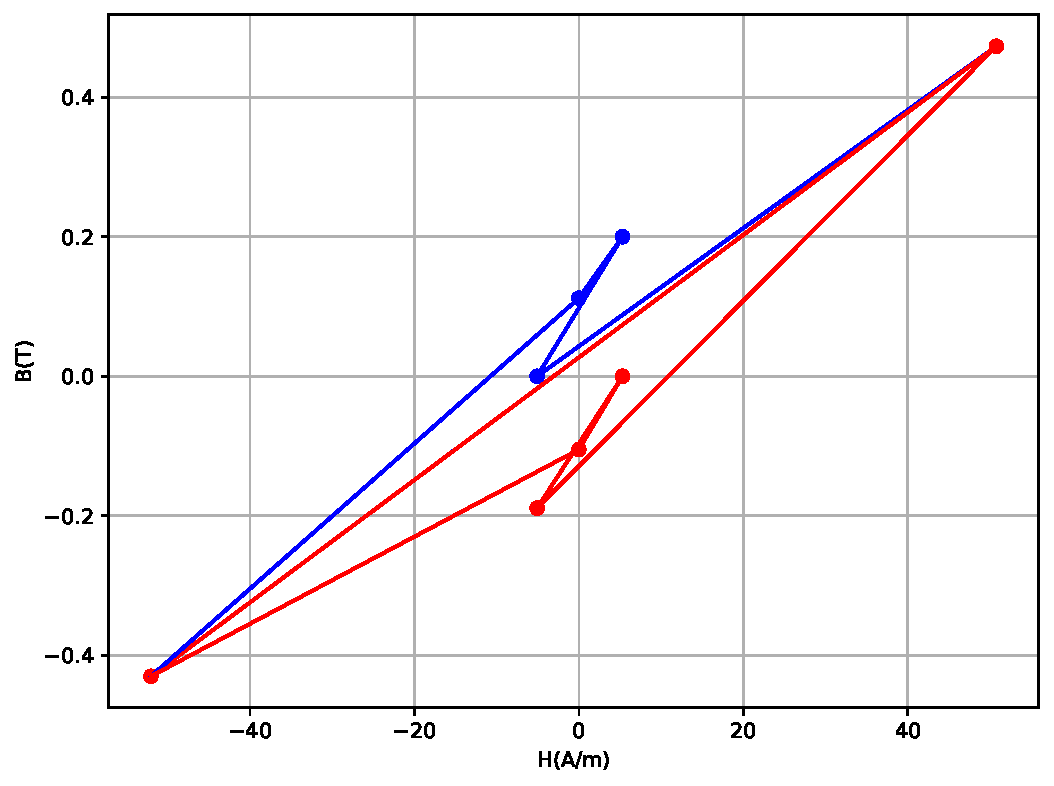
\includegraphics[width=0.5\textwidth]{table1.pdf} % PDF 文件名
    \caption{饱和磁滞回线} % 插图标题
    \label{fig:饱和磁滞回线} % 插图标签
\end{figure}
\begin{figure}[htbp]
    \centering
    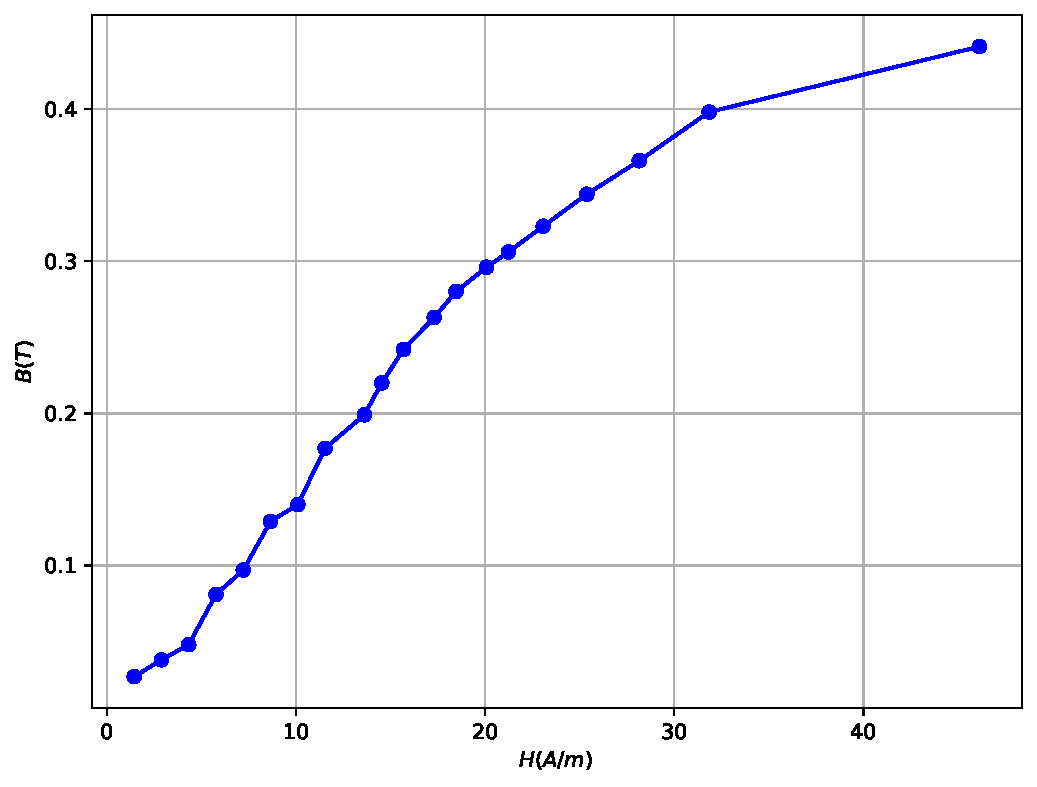
\includegraphics[width=0.4\textwidth]{table4_1.pdf} % PDF 文件名
    \caption{铁氧体的动态磁化曲线} % 插图标题
    \label{fig: 铁氧体的动态磁化曲线} % 插图标签
\end{figure}

\newpage
\begin{figure}[htbp]
    \centering
    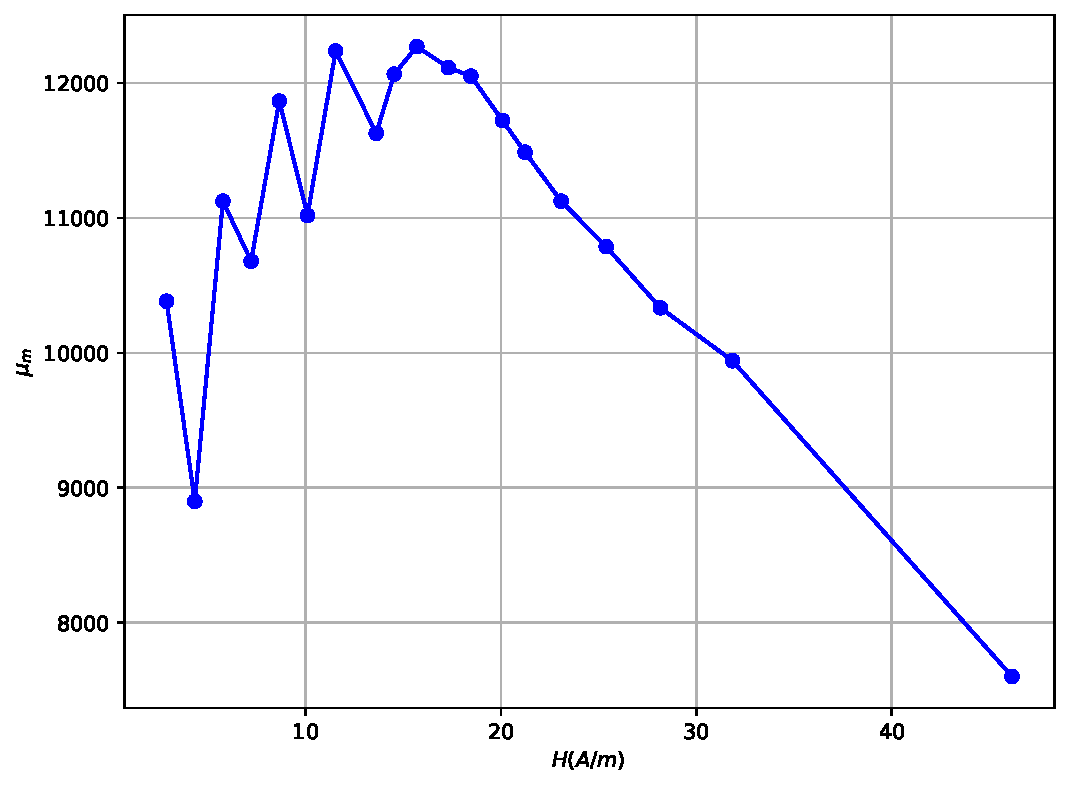
\includegraphics[width=0.4\textwidth]{table4_2.pdf} % PDF 文件名
    
    \caption{铁氧体的曲线} % 插图标题
    \label{fig:铁氧体的曲线} % 插图标签
\end{figure}

\begin{figure}[htbp]
    \centering
    
\includegraphics[width=0.4\textwidth]{table4_2_fitted.pdf} % PDF 文件名
    \caption{铁氧体的曲线(使用算法平滑拟合后的结果)} % 插图标题
    \label{fig:铁氧体的曲线（使用算法平滑拟合后的结果）} % 插图标签
\end{figure}

\newpage
\begin{figure}[htbp]
    \centering
    
\includegraphics[width=0.4\textwidth]{table6.pdf} % PDF 文件名
    \caption{样品1（铁氧体）在不同直流偏置磁场下的可逆磁导率} % 插图标题
    \label{fig:样品1（铁氧体）在不同直流偏置磁场下的可逆磁导率} % 插图标签
\end{figure}

\begin{figure}[htbp]
    \centering
    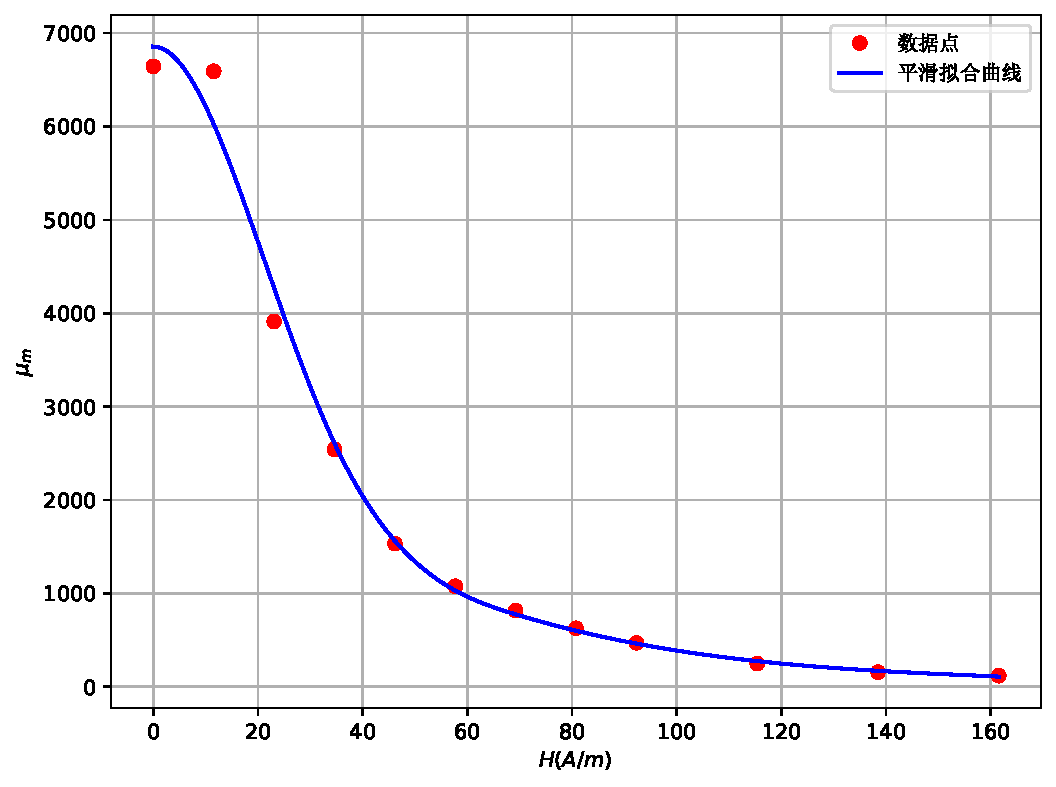
\includegraphics[width=0.4\textwidth]{table6_fitted.pdf} % PDF 文件名
    \caption{样品1（铁氧体）在不同直流偏置磁场下的可逆磁导率(使用算法拟合)} % 插图标题
    \label{fig:样品1（铁氧体）在不同直流偏置磁场下的可逆磁导率（使用算法拟合）} % 插图标签
\end{figure}


\newpage
\section{用霍尔传感器测量铁磁材料的准静态磁滞回线}

\subsection{实验内容}
\subsubsection{测量样品的起始磁化曲线}
\begin{enumerate}
    \item 选择合适的电流与磁感应强度 $B$，用数字式特斯拉计测量样品间隙中剩磁的磁感应强度 $B$ 与位置 $X$ 的关系，$X$ 从-10mm 到 10mm，间隔 1mm 测一组数据，求得间隙中磁感应强度 $B$ 的均匀区范围 $\Delta X$ 值，将霍尔传感器放在测出的均匀区的中央。
    \item 对样品进行退磁处理。其方法是利用双刀开关使磁化电流不断反向，且幅值由最大值逐渐减小至零，最终使样品的剩磁 $B$ 为零。例如将电流值由 0 增至 600mA 再逐渐减小至 0，然后双刀开关换为反向电流由 0 增至 500mA，再由 500mA 调至零，这样磁化电流不断反向，最大电流值每次减小 100mA，当剩磁减小到 100mT，每次最大电流减小量还需小些，最后将剩磁消除。然后测量 $B-H$ 关系曲线。利用公式$$H\bar l + \frac{1}{\mu_0}Bl_g=NI$$得到修正后的磁场，再利用读到的$B$数据绘图，测得的结果如图\ref{fig:测量样品的起始磁化曲线}所示。
\end{enumerate}
\subsubsection{测量模具钢的磁滞回线}
\begin{enumerate}
    \item 测量模具钢的磁滞回线前的磁锻炼。由初始磁化曲线可以得到 $B$ 增加得十分缓慢时，磁化线圈通过的电流值 $I_m$，然后保持此电流 $I_m$ 不变，把双刀换向开关来回拨动 8-10 次，进行磁锻炼。
    \item 测量模具钢的磁滞回线。通过磁化线圈的电流从饱和电流 $I_m$ 开始逐步减小到 0，然后双刀换向开关将电流换向，电流又从 0 增加到 $-I_m$，重复上述过程，即 $(H_m, B_m) \rightarrow (-H_m, -B_m)$，再从 $(-H_m, -B_m) \rightarrow (H_m, B_m)$。每隔 50mA 测一组 $(I_i, B_i)$ 值。利用公式$$H\bar l + \frac{1}{\mu_0}Bl_g = NI$$得到修正后的磁场，再利用读到的$B$数据绘图，结果如\ref{fig:测量模具钢的磁滞回线}所示。
\end{enumerate}

\subsection{数据整理与计算}
\subsubsection{测量样品的起始磁化曲线}

\begin{table}[H]
  \centering
  \caption{测量样品的起始磁化曲线}\label{测量样品的起始磁化曲线}
        \begin{tabularx}{\textwidth}{|X|X|X|X|}
        \hline
        $I(mA)$ & $B(mT)$ & $H(A/m)$ & 修正$H(A/m)$ \\
        \hline
        0.000 & 4.500 & 0.000 & -29.842 \\
        \hline
        29.600 & 14.300 & 246.667 & 151.837 \\
        \hline
        60.200 & 25.800 & 501.667 & 330.575 \\
        \hline
        90.200 & 38.600 & 751.667 & 495.692 \\
        \hline
        120.100 & 52.600 & 1000.833 & 652.018 \\
        \hline
        150.400 & 68.400 & 1253.333 & 799.741 \\
        \hline
        181.100 & 89.500 & 1509.167 & 915.651 \\
        \hline
        211.300 & 110.900 & 1760.833 & 1025.404 \\
        \hline
        240.700 & 131.500 & 2005.833 & 1133.796 \\
        \hline
        270.600 & 153.200 & 2255.000 & 1239.060 \\
        \hline
        300.000 & 174.900 & 2500.000 & 1340.157 \\
        \hline
        330.300 & 197.500 & 2752.500 & 1442.786 \\
        \hline
        360.000 & 219.900 & 3000.000 & 1541.742 \\
        \hline
        390.500 & 242.800 & 3254.167 & 1644.048 \\
        \hline
        420.600 & 264.900 & 3505.000 & 1748.326 \\
        \hline
        450.100 & 285.400 & 3750.833 & 1858.214 \\
        \hline
        482.000 & 306.500 & 4016.667 & 1984.124 \\
        \hline
        510.800 & 324.200 & 4256.667 & 2106.747 \\
        \hline
        540.000 & 340.800 & 4500.000 & 2239.998 \\
        \hline
        570.300 & 356.700 & 4752.500 & 2387.058 \\
        \hline
        \end{tabularx}
\end{table}

\subsubsection{测量模具钢的磁滞回线}

%\renewcommand{\arraystretch}{1.3} % 增加行距

\begin{longtable}{|p{0.22\textwidth}|p{0.22\textwidth}|p{0.23\textwidth}|p{0.23\textwidth}|}
  \caption{测量模具钢的磁滞回线} \label{测量模具钢的磁滞回线} \\
  \hline
  $I(mA)$ & $B(mT)$ & $H(A/m)$ & 修正$H(A/m)$ \\
  \hline
  \endfirsthead

  \hline
  $I(mA)$ & $B(mT)$ & $H(A/m)$ & 修正$H(A/m)$ \\
  \hline
  \endhead

  \hline
  \endfoot

  633.200 & 395.900 & 5276.667 & 2651.271 \\
  \hline
  578.900 & 388.900 & 4824.167 & 2245.191 \\
  \hline
  530.000 & 381.700 & 4416.667 & 1885.438 \\
  \hline
  479.000 & 372.900 & 3991.667 & 1518.795 \\
  \hline
  430.100 & 362.600 & 3584.167 & 1179.599 \\
  \hline
  380.600 & 349.700 & 3171.667 & 852.645 \\
  \hline
  330.100 & 332.600 & 2750.833 & 545.209 \\
  \hline
  280.600 & 310.900 & 2338.333 & 276.612 \\
  \hline
  230.100 & 282.900 & 1917.500 & 41.460 \\
  \hline
  179.500 & 249.500 & 1495.833 & -158.716 \\
  \hline
  129.300 & 212.600 & 1077.500 & -332.349 \\
  \hline
  80.200  & 174.100 & 668.333  & -486.204 \\
  \hline
  30.300  & 133.500 & 252.500  & -632.800 \\
  \hline
  0.000   & 108.100 & 0.000    & -716.861 \\
  \hline
  -51.700 & 64.100  & -430.833 & -855.910 \\
  \hline
  -100.300 & 22.300  & -835.833 & -983.715 \\
  \hline
  -150.200 & -20.900 & -1251.667 & -1113.069 \\
  \hline
  -200.300 & -64.300 & -1669.167 & -1242.764 \\
  \hline
  -250.200 & -106.200 & -2085.000 & -1380.739 \\
  \hline
  -300.500 & -147.300 & -2504.167 & -1527.352 \\
  \hline
  -350.200 & -186.900 & -2918.333 & -1678.913 \\
  \hline
  -400.000 & -224.900 & -3333.333 & -1841.918 \\
  \hline
  -450.900 & -261.600 & -3757.500 & -2022.710 \\
  \hline
  -500.400 & -294.700 & -4170.000 & -2215.708 \\
  \hline
  -550.500 & -324.400 & -4587.500 & -2436.254 \\
  \hline
  -602.700 & -351.300 & -5022.500 & -2692.868 \\
  \hline
  -633.300 & -365.000 & -5277.500 & -2857.017 \\
  \hline
  -580.500 & -358.000 & -4837.500 & -2463.437 \\
  \hline
  -530.300 & -350.700 & -4419.167 & -2093.513 \\
  \hline
  -480.300 & -342.300 & -4002.500 & -1732.551 \\
  \hline
  -430.400 & -332.100 & -3586.667 & -1384.358 \\
  \hline
  -380.500 & -319.400 & -3170.833 & -1052.745 \\
  \hline
  -330.000 & -303.100 & -2750.000 & -740.004 \\
  \hline
  -280.100 & -282.100 & -2334.167 & -463.431 \\
  \hline
  -230.200 & -255.500 & -1918.333 & -223.995 \\
  \hline
  -179.900 & -223.300 & -1499.167 & -18.361 \\
  \hline
  -127.800 & -185.700 & -1065.000 & 166.462 \\
  \hline
  -78.200  & -147.400 & -651.667  & 325.811 \\
  \hline
  -30.900  & -109.400 & -257.500  & 467.982 \\
  \hline
  0.000    & -83.600  & 0.000     & 554.390 \\
  \hline
  49.700   & -41.900  & 414.167   & 692.025 \\
  \hline
  100.100  & 1.000    & 834.167   & 827.535 \\
  \hline
  150.200  & 44.700   & 1251.667  & 955.240 \\
  \hline
  201.100  & 88.600   & 1675.833  & 1088.286 \\
  \hline
  250.400  & 129.900  & 2086.667  & 1225.240 \\
  \hline
  300.700  & 170.900  & 2505.833  & 1372.517 \\
  \hline
  350.200  & 210.200  & 2918.333  & 1524.400 \\
  \hline
  400.100  & 248.400  & 3334.167  & 1686.912 \\
  \hline
  450.000  & 284.300  & 3750.000  & 1864.675 \\
  \hline
  501.300  & 318.000  & 4177.500  & 2068.695 \\
  \hline
  551.400  & 347.000  & 4595.000  & 2293.883 \\
  \hline
  601.000  & 371.600  & 5008.333  & 2544.082 \\
  \hline
  633.300  & 385.700  & 5277.500  & 2719.745 \\
  \hline
\end{longtable}
\subsection{绘图}
\subsubsection{测量样品的起始磁化曲线}

\begin{figure}[htbp]
    \centering
    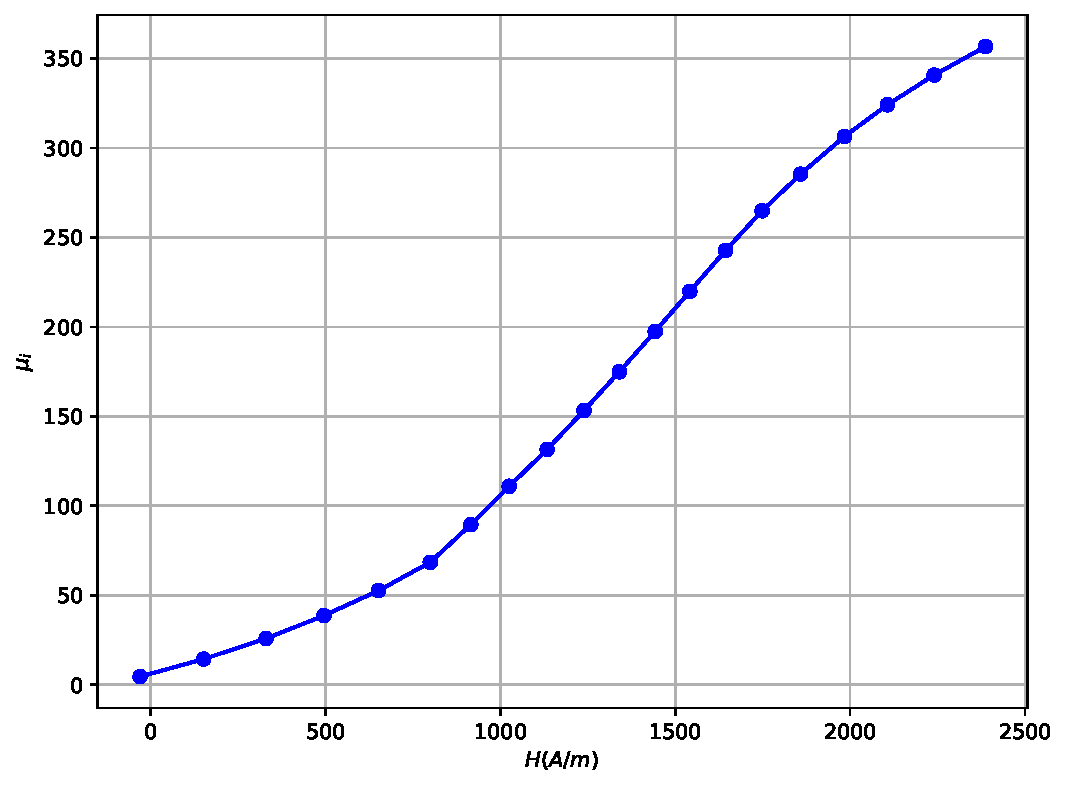
\includegraphics[width=0.4\textwidth]{table7.pdf} % PDF 文件名
    \caption{测量样品的起始磁化曲线} % 插图标题
    \label{fig:测量样品的起始磁化曲线} % 插图标签
\end{figure}

\subsubsection{测量模具钢的磁滞回线}

\begin{figure}[htbp]
    \centering
    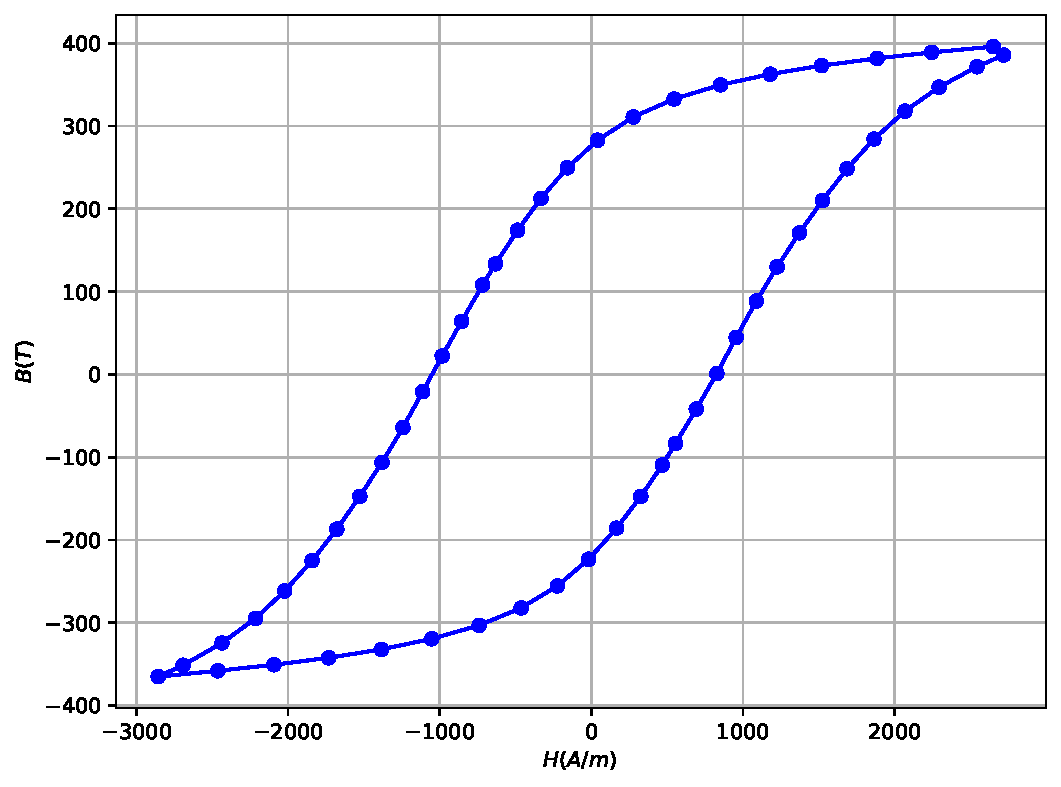
\includegraphics[width=0.4\textwidth]{table8.pdf} % PDF 文件名
    \caption{测量模具钢的磁滞回线} % 插图标题
    \label{fig:测量模具钢的磁滞回线} % 插图标签
\end{figure}

\newpage
\section{思考题与实验心得}
\subsection{思考题}
\textbf{1. 铁磁材料的动态磁滞回线与（准）静态磁滞回线在概念上有什么区别？铁磁材料动态磁滞回线的形状和面积受哪些因素影响？}

动态磁滞回线和准静态磁滞回线的主要区别在于磁化过程的频率：
\begin{itemize}
    \item 动态磁滞回线是在交流磁场下进行的，除磁滞损耗外，还有涡流损耗等损耗。其形状和面积与材料自身的性质、磁场的频率、幅度和电阻与电容的取值有关。
    \item 准静态磁滞回线则是在接近静态的条件下测量的，主要表现磁滞损耗。由于频率较低，涡流损耗等损耗较少。
\end{itemize}

动态磁滞回线的形状和面积主要受以下因素影响：
\begin{itemize}
    \item \textbf{磁场的频率}：频率越高，剩磁和矫顽力下降，磁滞回线面积较小。
    \item \textbf{积分常量}：不同积分常量下李萨如图形的样貌不同。
    \item \textbf{材料特性}：材料自身的性质会影响磁滞回线的形状和面积。
\end{itemize}

\textbf{2. 什么叫做基本磁化曲线？它和起始磁化曲线间有何区别？}

基本磁化曲线是在样品经过磁锻炼之后，通过测量磁化过程中不同磁场强度下的磁感应强度得到的曲线，反映了材料在磁化过程中从未磁化状态到饱和状态的磁化特性。
\begin{itemize}
    \item 起始磁化曲线是材料从完全未磁化状态开始，随着外加磁场的增加，磁感应强度逐渐增加的曲线。它显示了材料在最初磁化时的磁化过程。
\end{itemize}
区别在于：
\begin{itemize}
    \item 起始磁化曲线只代表材料在第一次磁化时的特性，而基本磁化曲线是在样品经过反复磁化后，达到磁稳定状态后得到的。
\end{itemize}

\textbf{3. 铁氧体和硅钢材料的动态磁化特性各有什么特点？}

\begin{itemize}
    \item \textbf{铁氧体材料}具有较高的电阻率，因此在高频下涡流损耗小，适合用于高频设备。它的磁导率相对较低，但涡流损耗小。
    \item \textbf{硅钢材料}具有较低的电阻率，因此在高频磁化时会有较大的涡流损耗，适合用于低频应用。硅钢的磁导率较高，因此在低频下能够有效增强磁感应强度。
\end{itemize}

\textbf{4. 动态磁滞回线测量实验中，电路参量应怎样设置才能保证 \( u_{R1} - u_C \) 所形成的李萨如图形正确反映材料动态磁滞回线的形状？}

为了确保李萨如图能够正确反映材料的动态磁滞回线，电路参数需要满足以下要求：
\begin{itemize}
    \item \textbf{电阻 \( R_1 \) 和电容 \( C \)} 的选值应确保积分电路能够准确反映磁感应强度的变化。
    \item \textbf{频率调节}：信号源频率应调整到适当范围（如实验中提到的 100 Hz），以确保磁滞回线清晰、对称。
    \item \textbf{电流和磁场调节}：应调整励磁电流和直流偏置，确保在示波器上调出清晰的李萨如图。
\end{itemize}

\textbf{5. 准静态磁滞回线测量实验中，为什么要对样品进行磁锻炼才能获得稳定的饱和磁滞回线？}

磁锻炼是为了确保样品达到磁稳定状态，消除样品中的剩磁，从而获得稳定的饱和磁滞回线。通过反复改变磁化方向，可以使材料中的磁畴重新排列，消除内部应力和历史磁化效应，从而保证测量得到的磁滞回线是对称且稳定的。

如果不进行磁锻炼，样品可能会保留一些历史磁化效应，导致测量结果不稳定，影响饱和磁滞回线的精确性。


\end{document}

% VScode 常用快捷键：

% F2:                       变量重命名
% Ctrl + Enter:             行中换行
% Alt + up/down:            上下移行
% 鼠标中键 + 移动:           快速多光标
% Shift + Alt + up/down:    上下复制
% Ctrl + left/right:        左右跳单词
% Ctrl + Backspace/Delete:  左右删单词    
% Shift + Delete:           删除此行
% Ctrl + J:                 打开 VScode 下栏(输出栏)
% Ctrl + B:                 打开 VScode 左栏(目录栏)
% Ctrl + `:                 打开 VScode 终端栏
% Ctrl + 0:                 定位文件
% Ctrl + Tab:               切换已打开的文件(切标签)
% Ctrl + Shift + P:         打开全局命令(设置)

% Latex 常用快捷键：

% Ctrl + Alt + J:           由代码定位到PDF


